\documentclass[tikz,border=12pt]{standalone}
\usepackage{tikz}
\usepackage{fontawesome5}
\usepackage{booktabs}
\usetikzlibrary{automata, positioning, arrows.meta, fit, backgrounds}
\begin{document}
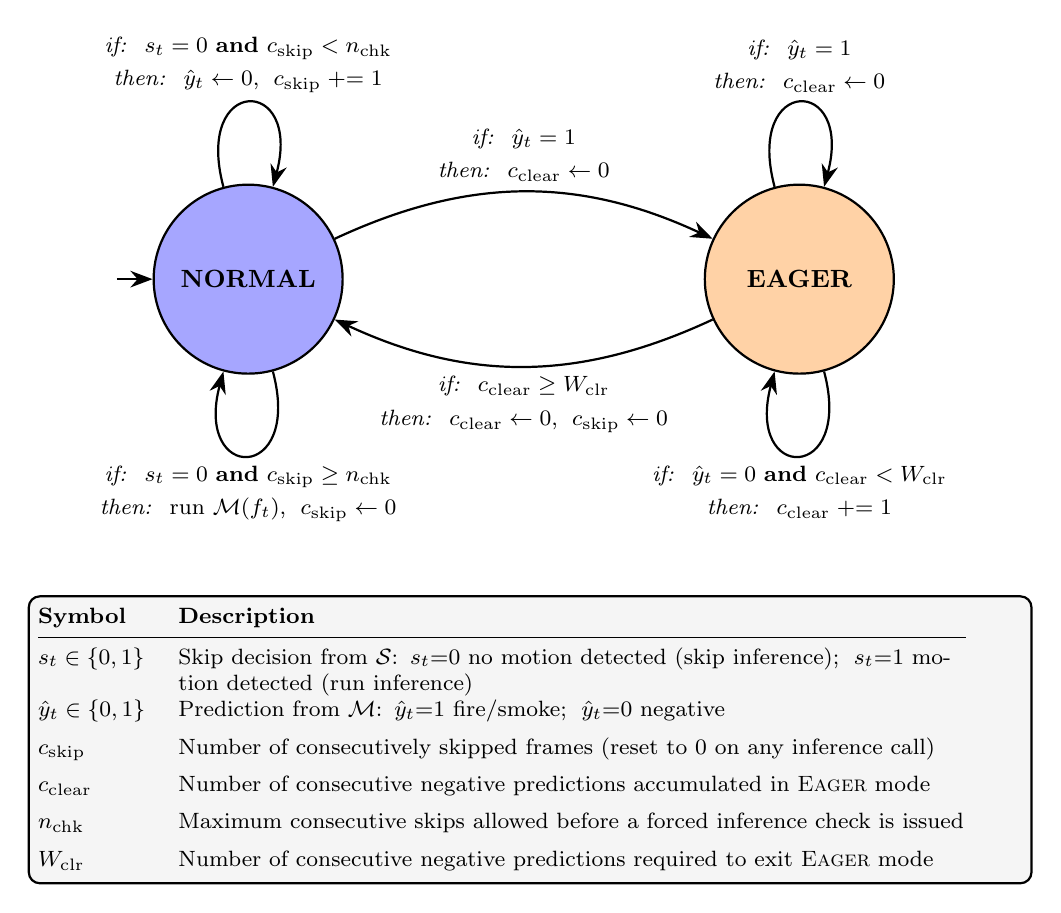
\begin{tikzpicture}[
        node distance=7cm,
        every state/.style={draw, rounded corners, minimum width=2.4cm,
        minimum height=1.2cm, font=\small\bfseries},
        thick,
        >={Stealth[length=8pt, width=6pt]},
        auto,
        label style/.style={font=\footnotesize, align=center}
    ]

    %% ── States ───────────────────────────────────────────────────────
    \node[state, initial, initial text={}, fill=blue!35] (normal) {NORMAL};
    \node[state, right of=normal, fill=orange!35]        (eager)  {EAGER};

    %% ── NORMAL → EAGER ───────────────────────────────────────────────
    %% guard / action
    \draw[->] (normal) edge[bend left=25]
    node[above, align=center]{%
        \footnotesize \textit{if:}\; $\hat{y}_t = 1$\\
    \footnotesize \textit{then:}\; $c_{\mathrm{clear}} \leftarrow 0$}
    (eager);

    %% ── EAGER → NORMAL ───────────────────────────────────────────────
    \draw[->] (eager) edge[bend left=25]
    node[below, align=center]{%
        \footnotesize \textit{if:}\; $c_{\mathrm{clear}} \geq
        W_{\mathrm{clr}}$\\
        \footnotesize \textit{then:}\; $c_{\mathrm{clear}} \leftarrow 0$,\;
    $c_{\mathrm{skip}} \leftarrow 0$}
    (normal);

    %% ── NORMAL self-loop: SKIP ───────────────────────────────────────
    \draw[->] (normal) edge[loop above, looseness=6]
    node[above, align=center]{%
        \footnotesize \textit{if:}\;
        $s_t = 0$ \textbf{and} $c_{\mathrm{skip}} < n_{\mathrm{chk}}$\\
        \footnotesize \textit{then:}\;
        $\hat{y}_t \leftarrow 0$,\;
    $c_{\mathrm{skip}} \mathrel{+}= 1$}
    (normal);

    %% ── NORMAL self-loop: FORCED CHECK ──────────────────────────────
    \draw[->] (normal) edge[loop below, looseness=6]
    node[below, align=center]{%
        \footnotesize \textit{if:}\;
        $s_t = 0$ \textbf{and} $c_{\mathrm{skip}} \geq n_{\mathrm{chk}}$\\
        \footnotesize \textit{then:}\;
        run $\mathcal{M}(f_t)$,\;
    $c_{\mathrm{skip}} \leftarrow 0$}
    (normal);

    %% ── EAGER self-loop: fire continues ─────────────────────────────
    \draw[->] (eager) edge[loop above, looseness=6]
    node[above, align=center]{%
        \footnotesize \textit{if:}\; $\hat{y}_t = 1$\\
    \footnotesize \textit{then:}\; $c_{\mathrm{clear}} \leftarrow 0$}
    (eager);

    %% ── EAGER self-loop: counting clears ────────────────────────────
    \draw[->] (eager) edge[loop below, looseness=6]
    node[below, align=center]{%
        \footnotesize \textit{if:}\;
        $\hat{y}_t = 0$ \textbf{and} $c_{\mathrm{clear}} < W_{\mathrm{clr}}$\\
        \footnotesize \textit{then:}\;
    $c_{\mathrm{clear}} \mathrel{+}= 1$}
    (eager);

    %% ── Legend ───────────────────────────────────────────────────────
    \node[draw, rounded corners, fill=gray!8,
        below=2.8cm of normal, anchor=north west,
        xshift=-2.8cm,
        text width=12.5cm,
    font=\footnotesize] (legend)
    {
        % \textbf{Notation} \\[2pt]
        \begin{tabular}{@{}lp{10cm}@{}}
            \textbf{Symbol} & \textbf{Description} \\
            \midrule
            $s_t \in \{0,1\}$       & Skip decision from $\mathcal{S}$:
            $s_t{=}0$ no motion detected (skip inference);\;
            $s_t{=}1$ motion detected (run inference) \\[4pt]
            $\hat{y}_t \in \{0,1\}$ & Prediction from $\mathcal{M}$:
            $\hat{y}_t{=}1$ fire/smoke;\;
            $\hat{y}_t{=}0$ negative \\[4pt]
            $c_{\mathrm{skip}}$     & Number of consecutively skipped frames
            (reset to $0$ on any inference call) \\[4pt]
            $c_{\mathrm{clear}}$    & Number of consecutive negative predictions
            accumulated in \textsc{Eager} mode \\[4pt]
            $n_{\mathrm{chk}}$      & Maximum consecutive skips allowed before
            a forced inference check is issued \\[4pt]
            $W_{\mathrm{clr}}$      & Number of consecutive negative predictions
            required to exit \textsc{Eager} mode \\
            % \bottomrule
        \end{tabular}
    };

\end{tikzpicture}
\end{document}
